\section{Zielsetzung}
  Ziel des Versuches ist es, die Funktionsweise und das Prinzip der Wärmepumpe durch eine beispielhafte Messung zu zeigen.

\section{Theorie}
  \label{sec:Theorie}
  Bei der Wärmepumpe handelt es sich um eine Vorrichtung, welche es erlaubt die durch den zweiten Hauptsatz der Thermodynamik gegebene Flussrichtung(vom wärmeren zum kälteren Körper) durch
  mechanische Arbeit umzukehren. Die Wärmepumpe ist dabei wie in Abbildung \ref{fig:skizze} dargestellt aufgebaut.
  \begin{figure}
    \centering
    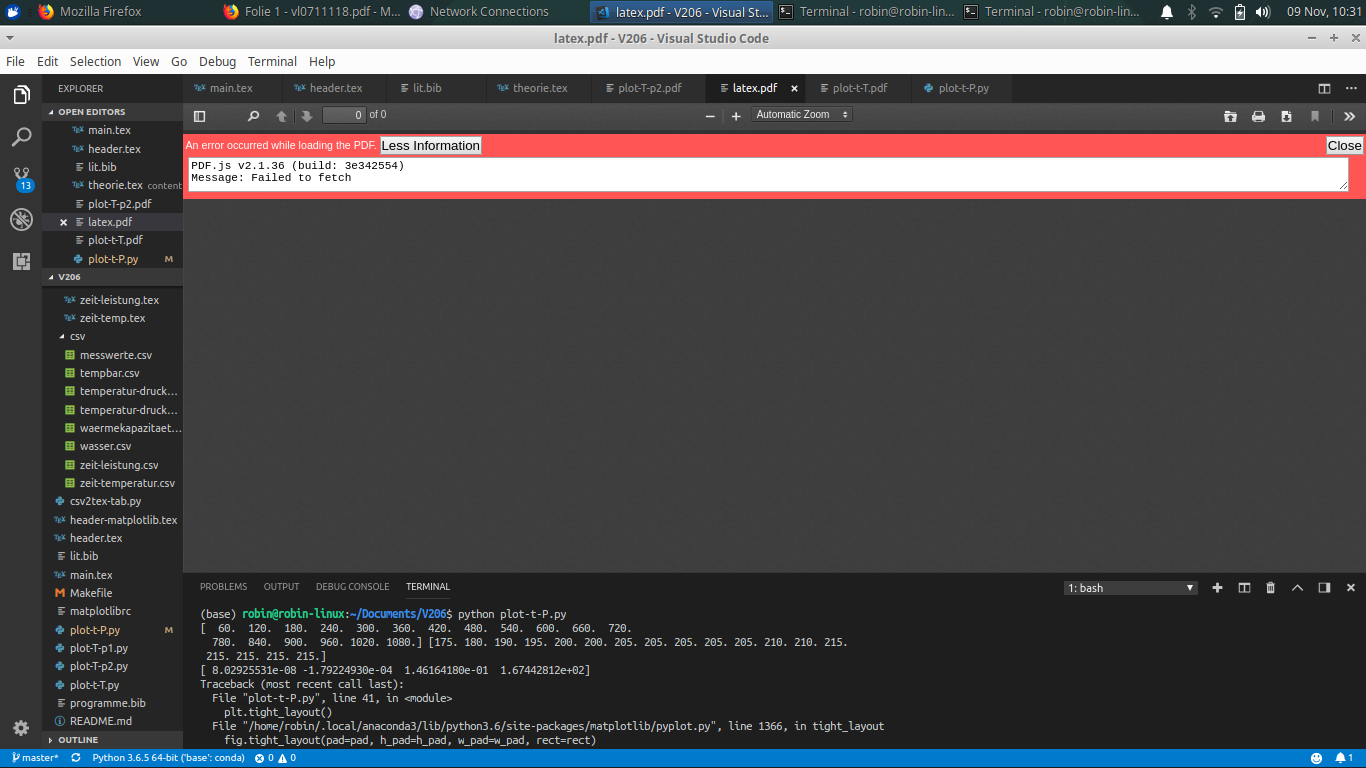
\includegraphics[width=\textwidth]{content/skizze.png}
    \caption{Schematischer Aufbau der Wärmepumpe \cite[193]{206}}
    \label{fig:skizze}
  \end{figure}
  Der Körper welcher in der Abbildung als Reservoir 1 bezeichnet wird, ist das Objekt, welches beheizt werden soll; das Reservoir 2 liefert die hierzu notwendige Energie.
  Wichtig ist, dass es sich bei den Reservoiren um abgeschlossene Systeme handelt, das heißt, dass sie möglichst thermisch isoliert sein müssen.
  Durch die beiden Reservoire wird ein reales Gas geleitet, in diesem Fall Dichlordifluormethan, welches die Eigenschaft besitzt den Agregatzustand durch sich verändernden Druck gut wechseln zu können.
  Bezogen auf Abbildung \ref{fig:skizze} heißt das, dass das Gas in Reservoir 2 einen Druck $p_2$ und eine Temperatur $T_2$ hat und gasförmig wird, wobei es dem Reservoir 2 die Verdampfungsenergie L entzieht. 
  Der Kompressor sorgt dabei für einen Gaskreislauf zwischen den Reservoiren und eine adiabatische Kompression, zwischen den Reservoiren, was heißt, dass dabei keine zusätzliche Wärme an die Umgebung abgegeben wird.
  Wenn das gasförmige Gas nun in Reservoir 1 strömt, wird es aufgrund des höheren Druckes $p_1 > p_2$, welcher durch die Kompression vorliegt, wieder flüssig und gibt dabei Wärmeenergie an das Reservoir mit Temperatur $T_1$ ab. Das nun flüssige Gas strömt dann durch ein Drosselventil zurück zu Reservoir 2 und der Kreislauf führt sich fort.
  Nach und nach erwärmt sich das Reservoir 1 also, während sich Reservoir 2 nach und nach weiter abkühlt.
  In der Praxis können Objekte so durch Reservoire geheizt werden, welche eine nahezu unendliche Menge konstanter Wärmeenergie aufweisen, wie die Umgebungsluft oder das Grundwasser.
  Weitere Bauteile neben dem Drosselventil, welches die Menge an einströmden flüssigen Gas reguliert, ein Steuergerät, welches die Regulierung des Drosselventils steuert und ein Reiniger welcher das flüssige Gas von gasförmigen Resten befreit, um den Kompressor zu entlasten.
  \subsection{Güteziffer}
    Die Güteziffer stellt die Effektivität der Wärmepumpe dar, das heißt das Verhältnis zwischen aufgebrachter mechanischer Arbeit A (für den Kompressor) und der transportierten Wärmemenge 

    Im folgenden bezeichnen A die mechanische Arbeit, $Q_1$ die abgebene Wärmemenge und $Q_2$ die aufgenomme Wärmemenge. 
    Nach dem ersten Hauptsatz der Thermodynamik muss die Energie im System erhalten bleiben, das heißt, dass sich die aufgenomme Wärme aus geleisteter Arbeit und abgegebener Wärme zusammensetzen muss, also
    \begin{equation}
      \label{eqt:gg}
      Q_1 = Q_2 + A .
    \end{equation}
    Bezogen auf die Temperatur, lässt sich mit Hilfe des zweiten Hauptsatz der Thermodynamik, welcher die Flussrichtung der Wärmeenergie durch den Fluss vom wärmeren zum kälteren Objekt bestimmt (Entropie), unter realistischen Annahmen,
    dass der Prozess irreversibel ist, da eine gewisse Verlustwärme bzw. Verlustenergie vorliegt,  
    muss folgende Relation gelten:
    \begin{equation}
      \label{eqt:güte_temp}
      \frac{Q_1}{T_1} - \frac{Q_2}{T_2} = 0 .
    \end{equation}
    Aus den Gleichungen \eqref{eqt:gg} und \eqref{eqt:güte_temp} lässt sich die Güte einer idealisierten Wärmepumpe als
    \begin{equation}
      \label{eqt:Güte}
      \nu_\text{ideal} = \frac {T_1}{T_1 - T_2}
    \end{equation}
    darstellen.
    Soll diese Güteziffer nun anhand einer Messreihe zu einer Wärmepumoe bestimmt werden, so muss zunächst, da hier mit einer Ausgleichsrechnung gearbeitet wird, der Differentialquotienten $\frac{\Delta T_1}{\Delta t }$
    erechnet werden und daraus ergibt sich dann für die abgebene Wärmemenge pro Zeiteinheit die Beziehung
    \begin{equation}
      \label{eqt:wärme_zeit}
      \frac{\Delta Q_1} {\Delta t} = (m_1 c_w + m_k c_k) \frac {\Delta T_1}{\Delta t},
    \end{equation}
    wobei $m_1 c_w$ die Wärmekapizität des Wassers im Reservoir und $m_k c_k$ die Wärmekapazitat der Rohre und der Reservoire sind.
    Die Güteziffer erechnet sich dann mit der über die Zeit $\Delta t$ gemittelte Leistung $P$ zu
    \begin{equation}
      \label{eqt:güte}
      \nu = \frac {\Delta Q_1}{\Delta t P}.
    \end{equation}
  \subsection{Massendurchsatz}
    Der Massendurchsatz bezeichnet die Masse an Gas, welche durch die Rohre strömt.
    Hierzu muss wie zuvor ein Differentialquotient gebildet werden. Für $\frac {\Delta T_2}{\Delta t}$ ergibt sich für die abgebene Wärmemenge pro Zeiteinheit $\Delta t$
    \begin{equation}
      \label{eqt:Diff_2}
      \frac {\Delta Q_2} {\Delta t} = (m_2 c_w + m_k c_k) \frac {\Delta T_2} {\Delta t}.
    \end{equation}
    Für die abgegebene Wärmemenge pro Zeiteinheit gilt außerdem, da die Abnahme der Wärme proportional zur bekannten Verdampfungswärme L geschieht, 
    \begin{equation}
      \label{eqt:verdampf}
      \frac {\Delta Q_2}{\Delta t} = L \frac {\Delta m} {\Delta t} .
    \end{equation}
    Werden \eqref {eqt:Diff_2} und \eqref {eqt:verdampf} zusammmengesetzt, so gilt für den Massendurchsatz:
    \begin{equation}
      \label{eqt:massendurchsatz}
      \frac {\Delta m} {\Delta t} = \frac {(m_2 c_w + m_k c_k)}{L} \frac {\Delta T_2} {\Delta t} .
    \end{equation}

  \subsection{Mechanische Kompressorleistung}
    Als mechanische Kompressorleistung P, wird die Leistung bezeichnet die benötigt wird um ein Gas mit dem Volumen $V_a$ auf ein Volumen $V_b$ zu verringern.
    Der Zusammenhang zur Arbeit $A_m$ besteht durch
    \begin{equation}
      P = \frac {\Delta A_m} {\Delta t},
    \end{equation}
    für welche gilt:
    \begin{equation}
      \label{eqt:mech_arbeit}
      A_m = - \int_{V_a}^{V_b} p \, \symup{d}V .
    \end{equation}
    Unter der Annahme, dass der Kompressor adiabatisch arbeitet, gilt die Poissongleichung für Druck $p_\text{a/b}$ und Volumen $V_\text{a/b}$:
    \begin{equation}
      \label{eqt:poisson}
      p_a V_a^\kappa = p_b V_b^\kappa = p V^\kappa .
    \end{equation}
    Mittels der Gleichungen \eqref {eqt:mech_arbeit} und \eqref {eqt:poisson} lässt sich die mechanische Leistung schließlich als
    \begin{equation}
      \label{eqt:mech_leistung}
      P = \frac {\Delta A_m} {\Delta t} = \frac {1}{\kappa -1} (p_b \sqrt[\kappa]{\frac{p_a}{p_b} - p_a } )  
    \end{equation}  
    darstellen, wobei $\rho$ die Dichte des Gases ist und $\frac {1}{\rho} \frac {\Delta m} {\Delta t} = \frac {\Delta V}{\Delta t}$